\documentclass[letter,11pt]{article}

\usepackage{fullpage}
\usepackage{hyperref}
\usepackage{graphicx}
\usepackage{multirow}
\usepackage{array}
\usepackage{adjustbox}

\graphicspath{{figures/}}

\newcommand{\niceurl}[1]{\href{#1}{\textsl{#1}}}
\newcommand{\code}[1]{\textsl{#1}}

\author{Dustin Lang}
\date{Aug 22, 2017}
\title{Evaluation of coadded and single-frame photometry methods}

\begin{document}
\maketitle

This report describes some simple experiments to evaluate the
signal-to-noise performance of coadding and single-frame photometry
methods.  The script for these experiments is publicly
available\footnote{%
  \niceurl{https://github.com/dstndstn/euclid/blob/master/coadd.py}}
and uses the \code{Tractor} code\footnote{%
  \niceurl{https://github.com/dstndstn/tractor}} to generate synthetic images.

The main question to be answered in this experiment is how much
signal-to-noise is lost (how much extra error is introduced) when
images are coadded before performing photometry, as compared to
performing photometry on single exposures and averaging the results at
``catalog level''.

This experiment assumes we are doing forced photometry on two
ground-based images.  That is, it assumes that we have a high-quality
catalog (eg, from Euclid VIS) in which we have detected a single point
source.  It assumes that we have correctly calibrated the astrometry
of the ground-based images, so we know exactly where in pixel
coordinates the point source will be found; and it also assumes that
we have a correct point-spread function (PSF) model for each image.
It assumes the two image were taken with the same bandpass filter, and
asks how well we can measure the flux of the point source in the
images.  We will vary the PSFs and the per-pixel noise.  In typical
ground-based images, the per-pixel noise is due primarily to the
Poisson distribution of the sky background, which is well approximated
by Gaussian noise; readout noise adds to this, but is usually fairly
small in comparison.  We will assume that the images have been
photometrically calibrated so that they are all in the same units;
thus longer exposures would result in the same measured flux values
but will have smaller per-pixel noise and smaller errors in the
measured fluxes.

We examine four cases, building up to the most realistic:
\begin{itemize}
\item \textbf{Case 1}: the two images have the same per-pixel noise,
  and the same PSF
\item \textbf{Case 2}: the two images have different levels of
  per-pixel noise, but the same PSF
\item \textbf{Case 3}: the two images have the same per-pixel noise
  but different PSFs
\item \textbf{Case 4}: the two images have different per-pixel noise
  and PSF (but the same per-image signal-to-noise).
\end{itemize}

For each of these four cases, we show results for three different
photometry methods.  In all cases, we are doing model-based forced
photometry: we are fitting for the flux where our pixel-space image
model best matches the observed pixels, given the per-pixel noise in
the images.
\begin{itemize}
  \item \textbf{Simultaneous fitting}: We do a single fit
    for the flux that produces the best match to both images at the
    same time.  That is, we are finding the flux that produces the
    smallest sum of chi-squared differences between the model and the
    images, summing the chi-squared of both images.
  \item \textbf{Single-frame averaging}: We fit for the flux
    in each image independently, and then compute a weighted average
    of the fluxes.  That is, we compute a best-fit flux for each
    image, and then average the flux measurements in ``catalog
    space''.
  \item \textbf{Coadding}: We add together the pixels of the
    two images (with weights), and then fit for the flux that best
    matches the coadded image.  When doing the fit, we compute the
    correct PSF model for the coadded images.  We test different
    \emph{coadd weights} $\alpha$, where the coadd is $C = \alpha A +
    (1 - \alpha) B$ for images $A$ and $B$, and the sum is pixelwise.
\end{itemize}

\begin{figure}[h!]
  \begin{center}
    \begin{tabular}{*{3}{c}}
      Simultaneous Fitting
      &
      Single-Frame Averaging
      &
      Coadding
      \\
      \adjustimage{width=0.2\textwidth,valign=T}{method-a}
      &
      \adjustimage{width=0.2\textwidth,valign=T}{method-b}
      &
      \adjustimage{width=0.2\textwidth,valign=T}{method-c}
      \\
    \end{tabular}
  \end{center}
  \caption{Schematics of the three photometry methods presented in
    this report.  In \emph{Simultaneous Fitting}, the flux is
    optimized to minimize the sum of chi-squared values between the
    model and data, summed over both images.  In \emph{Single-Frame
      Averaging}, we measure a flux for each image (by minimizing
    chi-squared in the single image), then weighted-average the two
    flux measurements.  In \emph{Coadding}, we compute a coadd
    (average the images), then fit a flux to the coadd.
    \label{fig:methods}
  }
\end{figure}

Note that the first method, Simultaneous Fitting, saturates the
Cram\'er--Rao bound, meaning that it extracts all the available
information in the images.  It is the most expensive in terms of
computation time and memory; it requires that all the images to be
measured are in memory at once.  We include it in this experiment only
for comparison; one of the results of this report is that Single-Frame
Averaging always performs exactly the same.  This is because the flux
measurements are sufficient statistics and are distributed as
Gaussians, so they can be combined at ``catalog level'' with simple
equations and no loss of information.  Single-Frame Averaging has the
strong advantage that each exposure is photometered independently, so
it is computationally cheap, can be distributed, and is embarrassingly
parallel.

\newpage

\section*{Case 1: Same noise, same PSF}

\begin{figure}[b!]
  \begin{center}
    %\begin{tabular}{cc}
    %\end{tabular}
    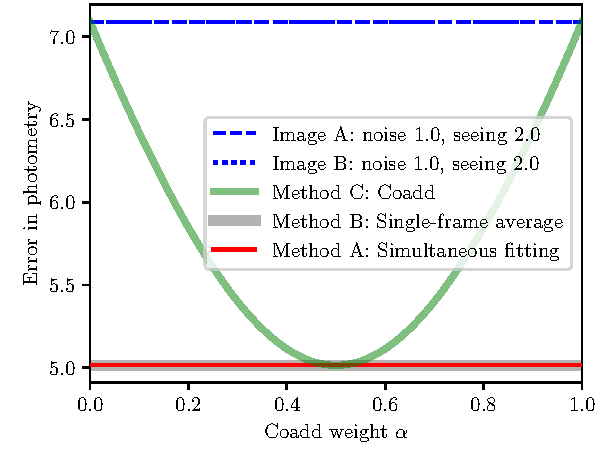
\includegraphics[width=0.48\textwidth]{coadd-00}
    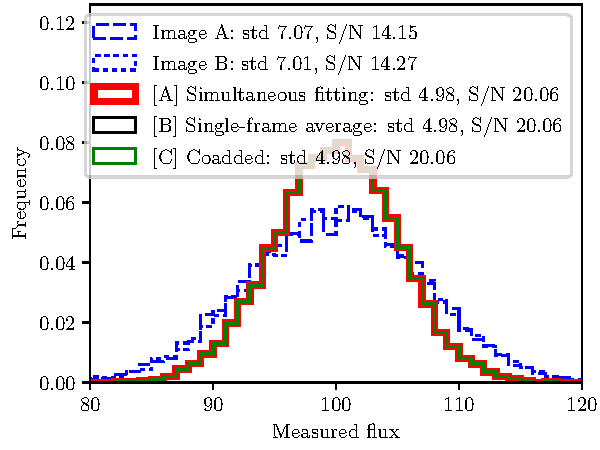
\includegraphics[width=0.48\textwidth]{coadd-01}
  \end{center}
  \caption{Results for Case 1 (same PSF, same per-pixel noise).  \textbf{Left}: the expected photometric
    uncertainty (error) for the different methods, as a function of
    the coadd weighting.  At the top of the plot, the two individual
    exposures, which have the same noise and PSF, have the same
    photometric error.  When the coadd weight is $\alpha = 0$ or $1$,
    the error in the coadd photometry equals that of the individual
    images.  With $\alpha = 0.5$, the coadd method performs as well as
    the other two methods.
    \newline \textbf{Right}: Results of simulations
    adding noise to synthetic images and running each of the
    photometry methods.  The measured fluxes are shown for $10,000$
    trials.  In this Case, the flux measurements on the individual
    exposures have a standard deviation of about 7, while all three
    of the other methods produce exactly the same results, with a standard
    deviation $1/\sqrt{2}$ as large; roughly 5.  Note that these results are
    entirely consistent with the analytically-computed expected performance values.
    \label{fig:caseone}}
\end{figure}


Figure~\ref{fig:caseone} shows results for Case 1.  In this case, all
three methods produce exactly the same results.  Since the two images
have the same PSF and per-pixel noise, the best coadd weight $\alpha =
0.5$.

\newpage

\section*{Case 2: Different noise, same PSF}

\begin{figure}[b!]
  \begin{center}
    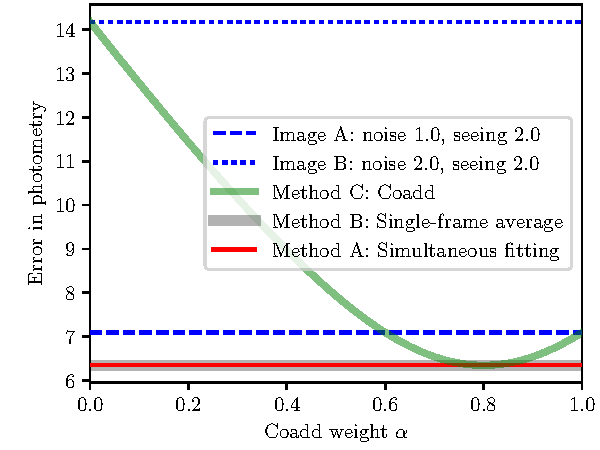
\includegraphics[width=0.48\textwidth]{coadd-02}
    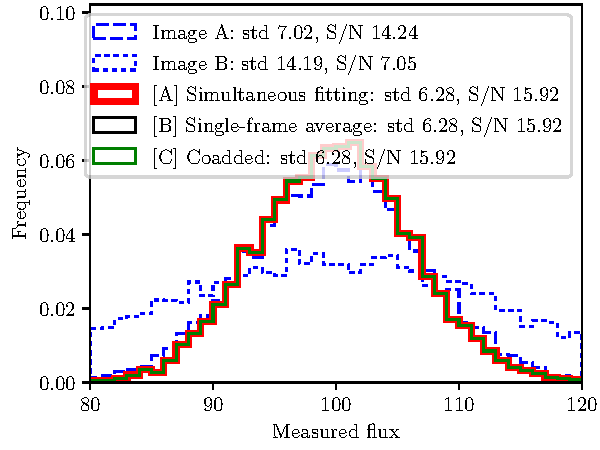
\includegraphics[width=0.48\textwidth]{coadd-03}
  \end{center}
  \caption{Results for Case 2 (same PSF, different per-pixel noise).
    \textbf{Left}: the expected photometric
    uncertainty (error) for the different methods, as a function of
    the coadd weighting.  Image A has half the per-pixel noise as Image B,
    so provides photometric measurements with half the uncertainty.
    The coadd weight that results in the best performance is $\alpha = 0.8$;
    this corresponds to inverse-variance weighting the images.
    \newline \textbf{Right}: Results of simulations where we
    add noise to synthetic images and run each of the
    photometry methods $10,000$ times.  The measured fluxes for
    the three methods are all identical, as in Case 1.
    \label{fig:casetwo}}
\end{figure}

In Case 2, one image has half the per-pixel noise as the other.
Results are shown in Figure~\ref{fig:casetwo}.  In this case, again,
each of the three methods produce the same results.  The best coadd
weight $\alpha$ is found to correspond to inverse-variance weighting
of the images: Image A, with half the noise, is given a weight four
times greater than that of Image B.

\newpage

\section*{Case 3: Same noise, different PSF}

\begin{figure}[b!]
  \begin{center}
    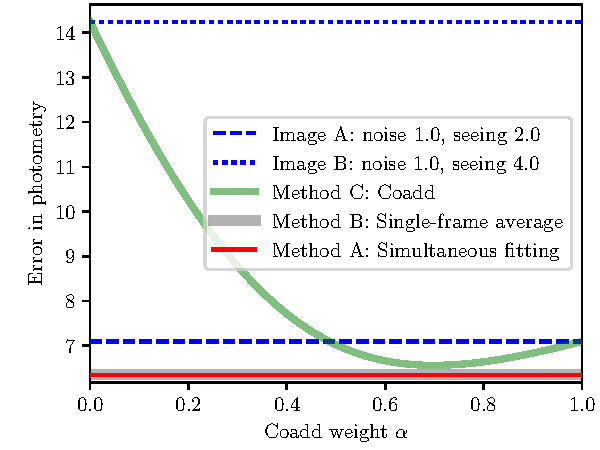
\includegraphics[width=0.48\textwidth]{coadd-04}
    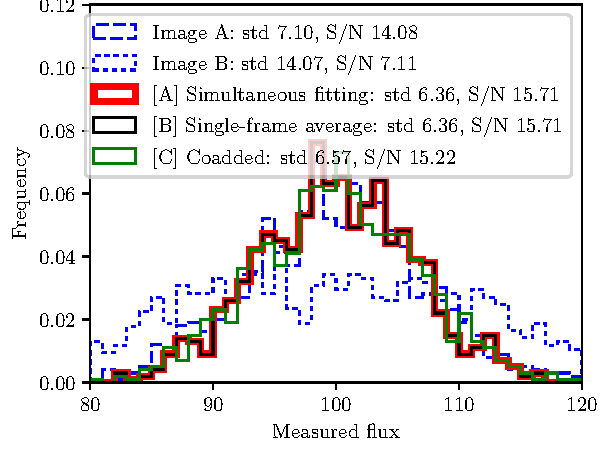
\includegraphics[width=0.48\textwidth]{coadd-05}
  \end{center}
  \caption{Results for Case 3 (same per-pixel noise, different PSF).
    \textbf{Left}: the expected photometric uncertainty (error) for
    the different methods, as a function of the coadd weighting.
    Image A has half the seeing size as Image B, and provides
    photometric measurements with half the uncertainty.  The coadd
    weight that results in the best performance is $\alpha \sim 0.7$.
    Even with the best coadd weight, the coadd method perform slightly
    worse than the other methods.  Since the majority of the
    signal-to-noise is carried by Image A, the difference is quite
    small.
    \newline \textbf{Right}: Results of simulations where we add noise
    to synthetic images and run each of the photometry methods
    $10,000$ times.  The measured fluxes for the three methods are as
    predicted: Simultaneous Fitting and Single-Frame Averaging still
    perform exactly the same, but Coadding performs slightly worse.
    \label{fig:casethree}}
\end{figure}

In Case 3, one image has half the seeing size (full-width at half-max,
FWHM) as the other.  Results are shown in Figure~\ref{fig:casethree}.
Here, the coadding method performs slightly worse than the other
methods.  This can be explained by the fact that optimal source
detection requires the use of a ``matched filter''---convolution by
the correct PSF---but in the coadded image, the two images with
different PSFs have been mixed together.  In other words, the matched
filters for the two images would place different relative weights on
the pixels; the PSF of the coadd places intermediate weights on
the pixels, so is less than optimal for both input images.

\newpage

\section*{Case 4: Different noise, different PSF}

\begin{figure}[b!]
  \begin{center}
    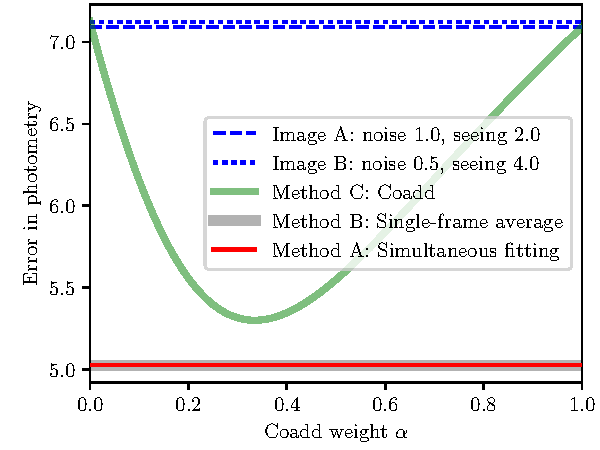
\includegraphics[width=0.48\textwidth]{coadd-06}
    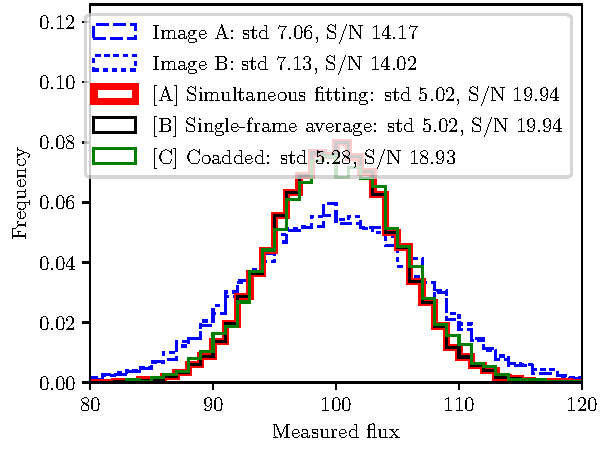
\includegraphics[width=0.48\textwidth]{coadd-07}
  \end{center}
  \caption{Results for Case 4 (different per-pixel noise, different
    PSF, same signal-to-noise).  \textbf{Left}: the expected
    photometric uncertainty (error) for the different methods, as a
    function of the coadd weighting.  Image A has half the seeing size
    as Image B, but more per-pixel noise, and thus provides
    photometric measurements with approximately equal uncertainty.
    (The signal-to-noise values are not exactly equal due to the
    effects of detector pixelization.)  The coadd weight that results
    in the best performance is $\alpha \sim 0.33$.  Even with the best
    coadd weight, the coadd method perform significantly worse than the
    other methods.
    \newline \textbf{Right}: Results of simulations where we add noise
    to synthetic images and run each of the photometry methods
    $10,000$ times.  The measured fluxes for the three methods are as
    predicted: Simultaneous Fitting and Single-Frame Averaging
    still perform exactly the same, but Coadding performs worse.
    \label{fig:casefour}}
\end{figure}

In Case 4, one image has half the seeing size (FWHM) as the other, but
the second image has half as much noise.  As such, the images are
equally sensitive.  This is a realistic case because many ground-based
surveys will take longer exposures (leading to less per-pixel noise)
when the seeing is worse, in order to produce a survey of uniform
depth.  The results for Case 4 are shown in Figure~\ref{fig:casefour}.
In this case, the coadd method produces significantly worse results.
Perhaps surprisingly, the best coadd weight $\alpha$ is not
$0.5$---equal weighting for the equally-sensitive images---but is
roughly $1/3$.  The loss of signal-to-noise from using the Coadding
method is roughly $5\%$, which may not seem like much, but observing
time goes with signal-to-noise squared, so this corresponds to more
than a $10\%$ increase in required observing time.


\newpage
\section*{Conclusions}

These experiments show that for the realistic case of different PSFs
and different per-pixel noise levels in ground-based images, creating
a coadd and then photometering it results in a significant ($5\%$)
less of signal-to-noise, or more than $10\%$ increase in required
telescope time.  On the other hand, performing photometry on
individual exposures and then computing weighted averages at ``catalog
level'' is shown to exactly match the signal-to-noise performance of
simultaneous fitting, and saturates the Cram\'er--Rao bound (that is,
extracts all available information).

Photometering individual exposures also has the programmatic advantage
that it is highly distributed: each input image is processed
independently, and updating the final photometric measurement when a
new images is taken is simple and fast.  A broader advantage is that
per-exposure information (such as spatially-varying filter response)
can be tagged on to single-exposure measurements and incorporated into
more advanced downstream processing, in which one would not summarize
the single-exposure measurements with a catalog-level average, but
instead forward-model the single-exposure measurements.

The code for this experiment is freely available.\footnote{%
  \niceurl{https://github.com/dstndstn/euclid/}}

\end{document}
